\chapter{Results \& Discussion}\label{chapter:results}
\chaptermark{Results \\ \& Discussion}

To asses and compare the different structures, we use the fitting parameters obtain from the model in \cref{eq:model}. To account for parameter correlations, we first determined the nonsaturable reflectivity by fitting the measurement with no pump power and then fixed the parameter for subsequent fits. This approach ensured that the fitting process accurately captures that the nonsaturable reflectivity stems from impurities of the structure, which don't change during a measurement. Additionally, we restricted the fitting range excluding high fluences. This was necessary since the exponential decrease in reflectivity in the model did not capture all the mechanism of inverse saturable absorption in the deep rollover.

In the subsequent sections, we go over of each of the three remaining fitting parameters. We explain the general trends and features of the measurements on the basis of the results for the copper heat spreader with pump DBR (cDBR) VECSEL design and then discuss these feature for the other structures. All the fitting parameters can be found in \cref{app:data}.

\begin{figure}[ht]
    \centering
    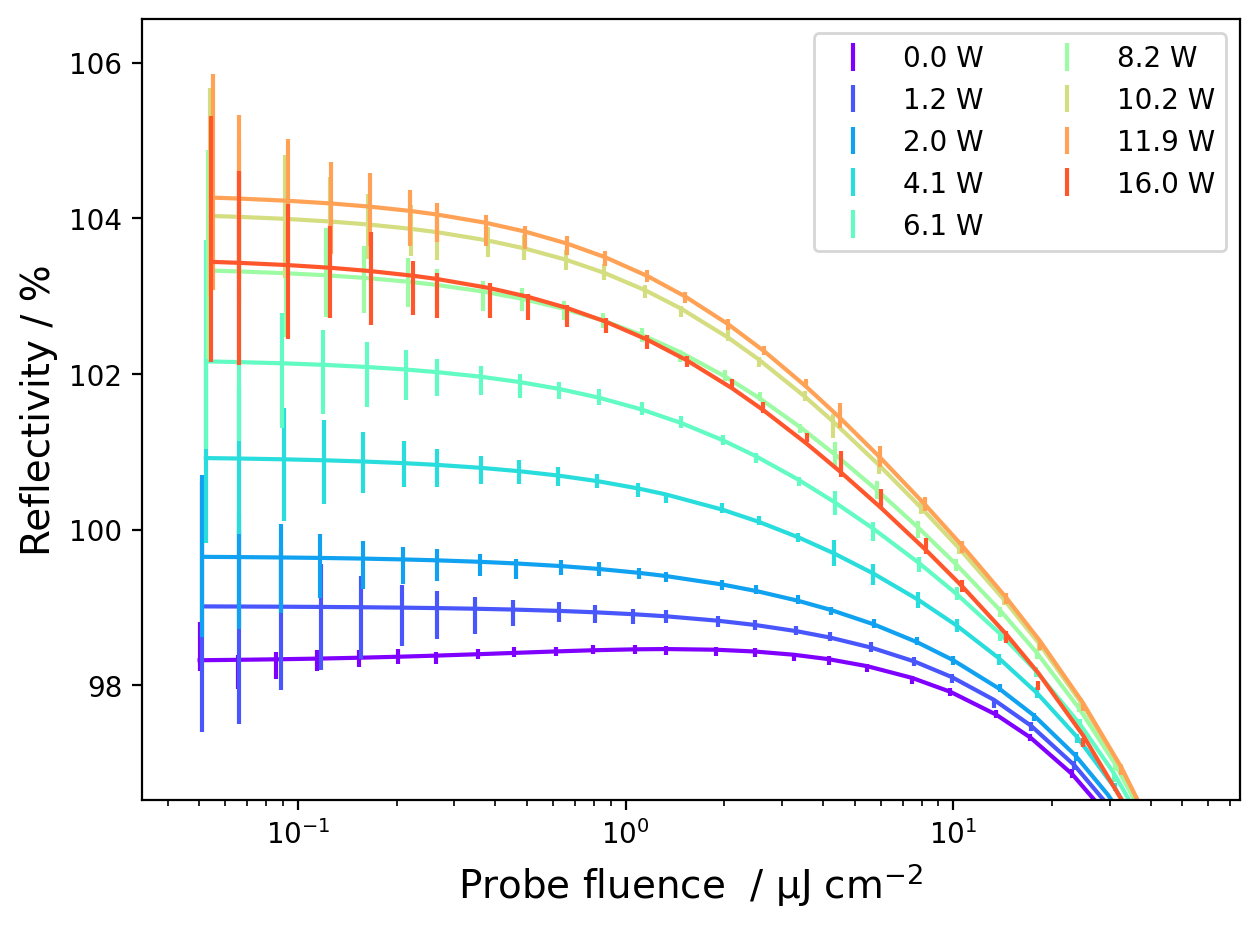
\includegraphics[width=8cm]{images/sv167-b5.png}
    \caption{Nonlinear reflectivity measurement for nine different pump powers of the pump DBR VECSEL with the copper heat spreader at \qty{0}{\celsius}. The data has been fitted with the model from \cref{eq:model}.}
    \label{fig:gainSV167}
\end{figure}

\section{\texorpdfstring{Saturation fluence $F_{sat}$}{Saturation fluence Fsat}}

\subsection*{Results}

\begin{wrapfigure}{r}{.48\textwidth}
    \vspace{-\baselineskip}
    \centering
    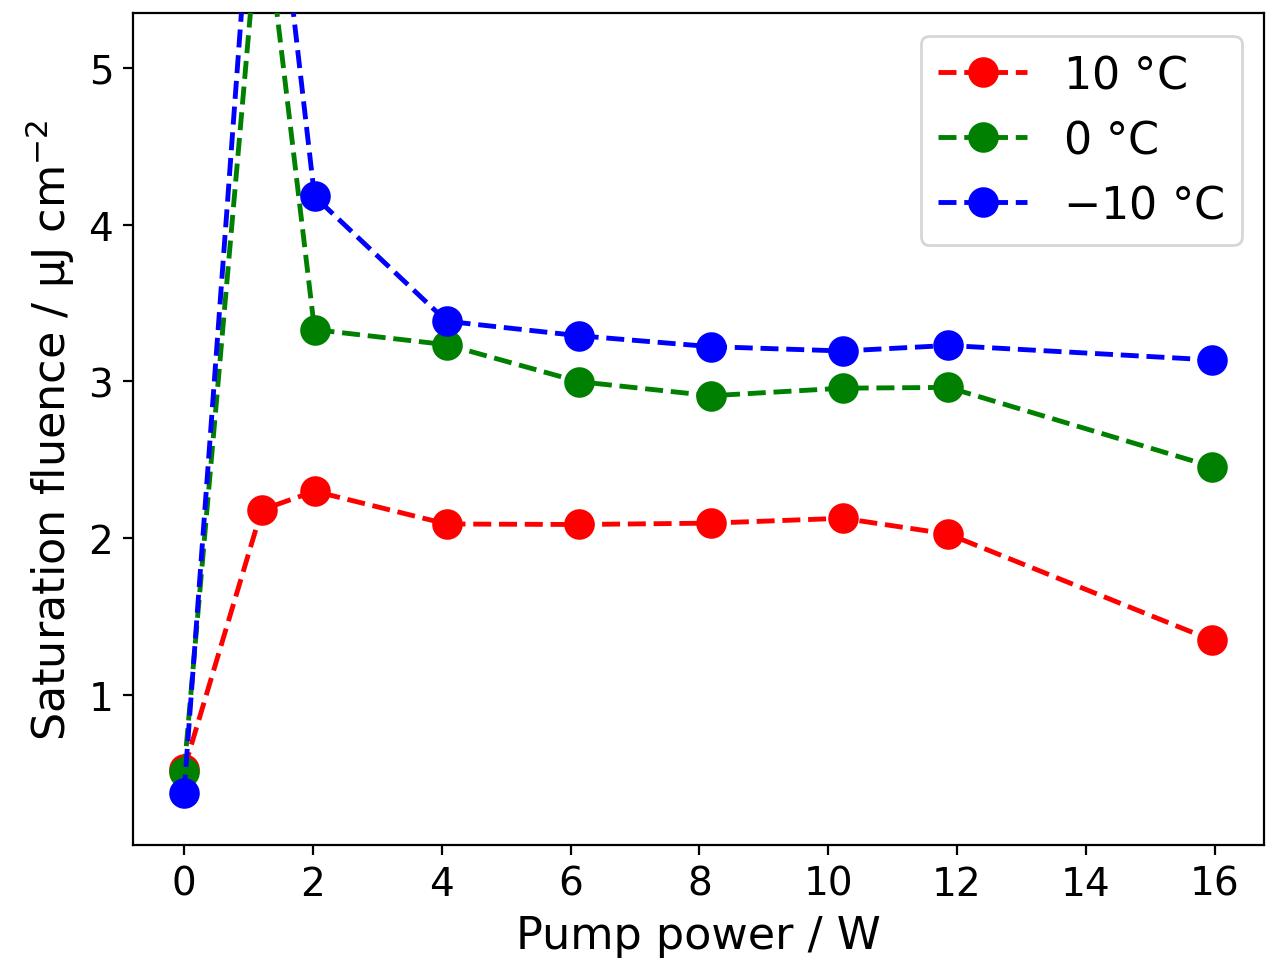
\includegraphics[width=.98\textwidth]{images/param0.png}
    \caption{Saturation fluences for the pump DBR VECSEL with a copper heat spreader.}
    \label{fig:fsat}
\end{wrapfigure}
In \cref{fig:fsat}, the saturation fluence of the cDBR VECSEL for three different heatsink temperatures.
Initially, at zero pump power, the saturation fluences are relatively low. But as soon as population inversion is reached within the gain region, the saturation fluence stays at a constant value. Before reaching the constant plateau, there is often a jump in the observed saturation fluence. This jump can be attributed to an an artifact from the fitting process. The flat reflectivity curve at low pump powers (see \cref{fig:gainSV167} for \qty{1.2}{\W}), makes it challenging for the fitting method to accurately determine the saturation fluence.

Regarding the temperature dependence we see that we get a higher saturation fluence for colder temperatures, which may appear counter intuitive considering that the carrier density decreases for lower temperatures. The explanation for this can be found in the design of the VECSEL. The optical thicknesses in the structure are designed for a specific wavelength, but thermal expansion/contraction can alter the thicknesses and therefore the specific wavelength of the design. %This effect had already been taken into account for in the design of the VECSEL. Meaning to reach the appropriate
As the measurements are performed for a fixed wavelength, the temperature can affect how much we are on resonance, hence modifying how efficient carriers can be promoted and therefore the observed saturation fluence. This nonlinear behaviour is also reflected in the data.


\subsection*{Discussion}
In \cref{tab:fsat} the mean values of the saturation fluences of the different structures and temperatures can be seen. The mean values were evaluated for data points with pump powers exceeding \qty{4}{\W} to minimize the influence of the fitting artifact.

Comparing the no pump DBR VECSEL to the cDBR VECSEL, no significant difference in the saturation fluence of the two structures is observed. This is reasonable considering that both chips have the same active region.

If we compare the two VECSEL with pump DBR we see that for \qty{10}{\celsius} they have the same saturation fluence. But for colder heat sink temperatures the VECSEL with the diamond heat spreader (dDBR) has a higher saturation fluence. This can be attributed to the improved thermal conductivity of the diamond heat spreader, resulting in a more efficient cooling of the structure. Consequently, the thermal expansion/contraction is also more significant and shifting the resonance of the structure enough to be more inline with the probing wavelength, therefore reaching a higher saturation fluence.

The hybrid VECSEL shows a different result compared to the others. In this case, cooling the structure moves the resonance of the design farther away from the probing wavelength, decreasing the saturation fluence.
\begin{table}[ht]
    \centering
    \begin{tabular}{llll}
        \multicolumn{4}{c}{Saturation fluence $F_{sat}$ / \unit{\micro\J\per\cm\squared}}                  \\ \hline
        Heat sink temperature                  &
        \multicolumn{1}{c}{\qty{10}{\celsius}} &
        \multicolumn{1}{c}{\qty{0}{\celsius}}  &
        \multicolumn{1}{c}{\qty{-10}{\celsius}}                                                            \\ \hline
        No pump DBR                            & \num{1.9\pm0.2}   & \num{3.5\pm0.2}   & \num{3.7\pm0.1}   \\ \hline
        Copper, pump DBR                       & \num{2.08\pm0.04} & \num{2.96\pm0.03} & \num{3.23\pm0.04} \\ \hline
        Diamond, pump DBR                      & \num{1.93\pm0.04} & \num{4.0\pm0.3}   & \num{4.3\pm0.3}   \\ \hline
        Hybrid                                 & \num{4.5\pm0.2}   & \num{1.83\pm0.02} & \num{1.6\pm0.03}
    \end{tabular}
    \caption{This table displays the mean saturation fluence values for the four VECSEL chips for the three heat sink temperatures. For the mean, only the values after the VECSEL achieved population inversion were used.}
    \label{tab:fsat}
\end{table}

\section{\texorpdfstring{Small signal reflectivity $R_{ss}$}{Small signal reflectivity Rss}}
\subsection*{Results}

\begin{wrapfigure}[16]{r}{.48\textwidth}
    \vspace{-\baselineskip}
    \centering
    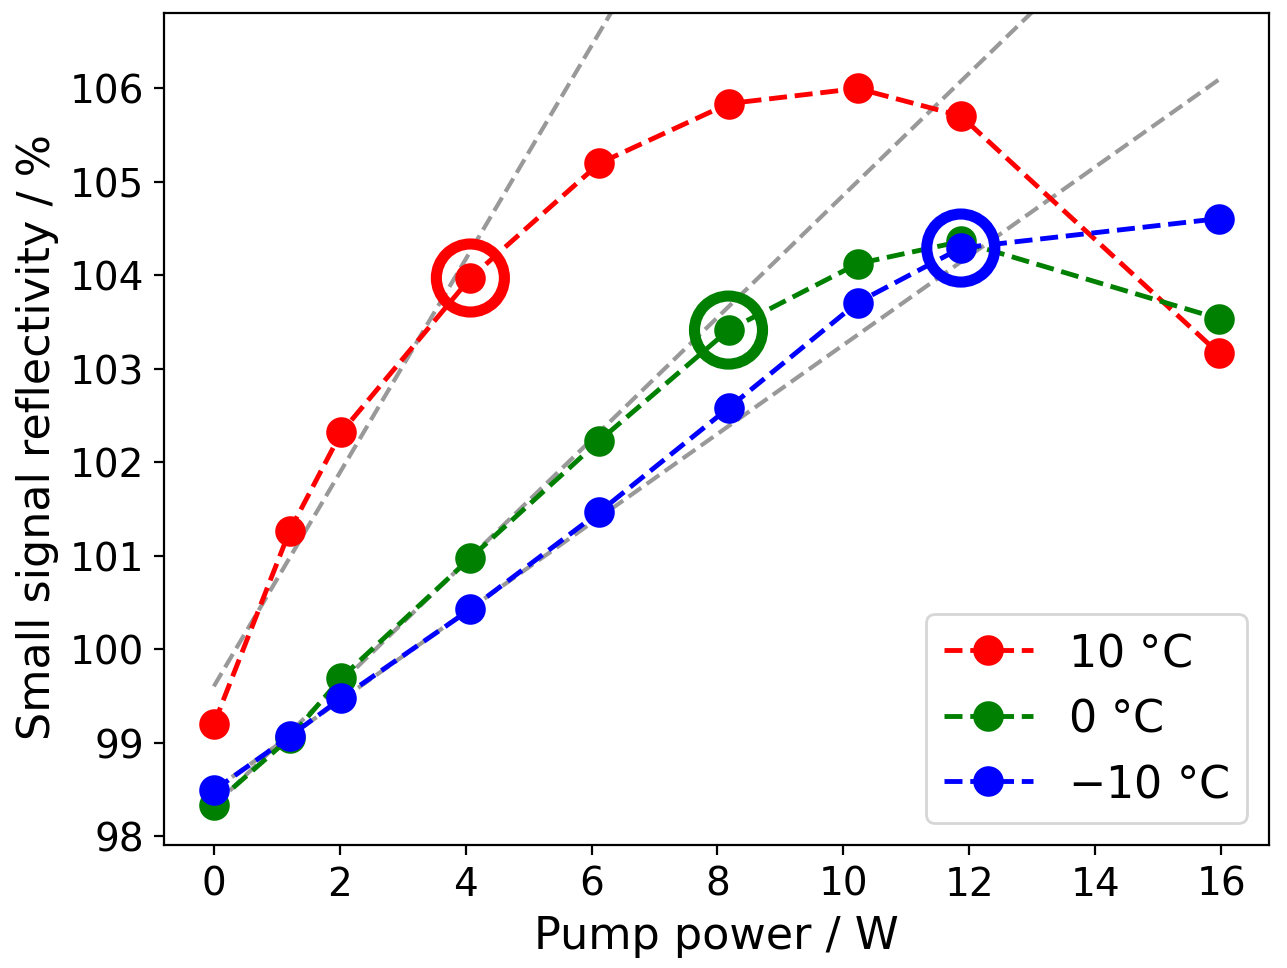
\includegraphics[width=.98\textwidth]{images/param1.png}
    \caption{Small signal reflectivity for the copper heat spreader pump DBR VECSEL. The break-off points are marked by circle around the data point.}
    \label{fig:rss}
\end{wrapfigure}

\cref{fig:rss} shows the small signal reflectivity for the cDBR VECSEL for the three different heatsink temperatures.
We see that the small signal reflectivity initially exhibits a linear growth but then drops off for higher pulse fluences. This break off tends to happen for higher fluence values for colder temperatures.

Notably for this measurement of the cDBR VECSEL, we see that the chips performance in terms of maximum reflectivity is higher compared to the colder temperatures. This can be most likely attributed to spatial variation in the measurement spot on the chip. Consequently, comparing maximum reflectivity values across different VECSEL lacks significance. Instead, we adopted a different approach to compare the chips by characterizing the break-off behaviour. For this, a linear regression for the first four data points was applied. The break-off point was determined as the power of the data point before deviating from the linear regression, referred to as the break-off power $P_{off}$.


\subsection*{Discussion}

In \cref{tab:rss} the break-off power $P_{off}$ and the maximum reflectivity $R_{max}$ are listed for the different VECSEL and heat sink temperatures. Comparing the different break-off powers to each other, there is no significant difference between the no pump DBR chip and the pump DBR chip. However, it shows that the break-off happens sooner for the diamond heat spreader than the copper, contrary to our expectation. This could be explained if we are limited with our gain by the material properties of the gain region and not some thermal effects, which could be investigated in the future. As for the maximum reflectivity, we observe that the dDDR chip shows overall higher performance compared to the other chips,  with a maximum small signal reflectivity of \qty{106.5}{\percent}.

\begin{table}[ht]
    \centering
    \begin{tabular}{lllllllll}
        \hline
        Heat sink temperature & \multicolumn{2}{c}{\qty{10}{\celsius}} &             & \multicolumn{2}{c}{\qty{0}{\celsius}} &           & \multicolumn{2}{c}{\qty{-10}{\celsius}}                              \\ \cline{2-3} \cline{5-6} \cline{8-9}
                              & $P_{off}$                              & $R_{max}$   &                                       & $P_{off}$ & $R_{max}$                               &  & $P_{off}$ & $R_{max}$   \\ 
                              & / \unit{\W} & / \unit{\percent} & &  / \unit{\W} & / \unit{\percent} & & / \unit{\W} & / \unit{\percent} \\ \hline
        No pump DBR           & 4                                      & \num{102.5} &                                       & 8         & \num{103.4}                             &  & 12        & \num{103.4} \\ \hline
        Copper, pump DBR      & 4                                      & \num{106.0} &                                       & 8         & \num{104.4}                             &  & 12        & \num{104.6} \\ \hline
        Diamond, pump DBR     & 4                                      & \num{105.3} &                                       & 6         & \num{106.2}                             &  & 10        & \num{106.5} \\ \hline
        Hybrid                & 6                                      & \num{103.5} &                                       & 10        & \num{103.6}                             &  & 12        & \num{103.7}
    \end{tabular}
    \caption{Break off power and maximum reflectivity values for the different measurement configurations.}
    \label{tab:rss}
\end{table}
\vspace{-2\baselineskip}

\section{\texorpdfstring{Rollover parameter $F_2$}{Rollover parameter F2}}
\subsection*{Results}

\begin{wrapfigure}[11]{r}{.48\textwidth}
    \vspace{-1.5\baselineskip}
    \centering
    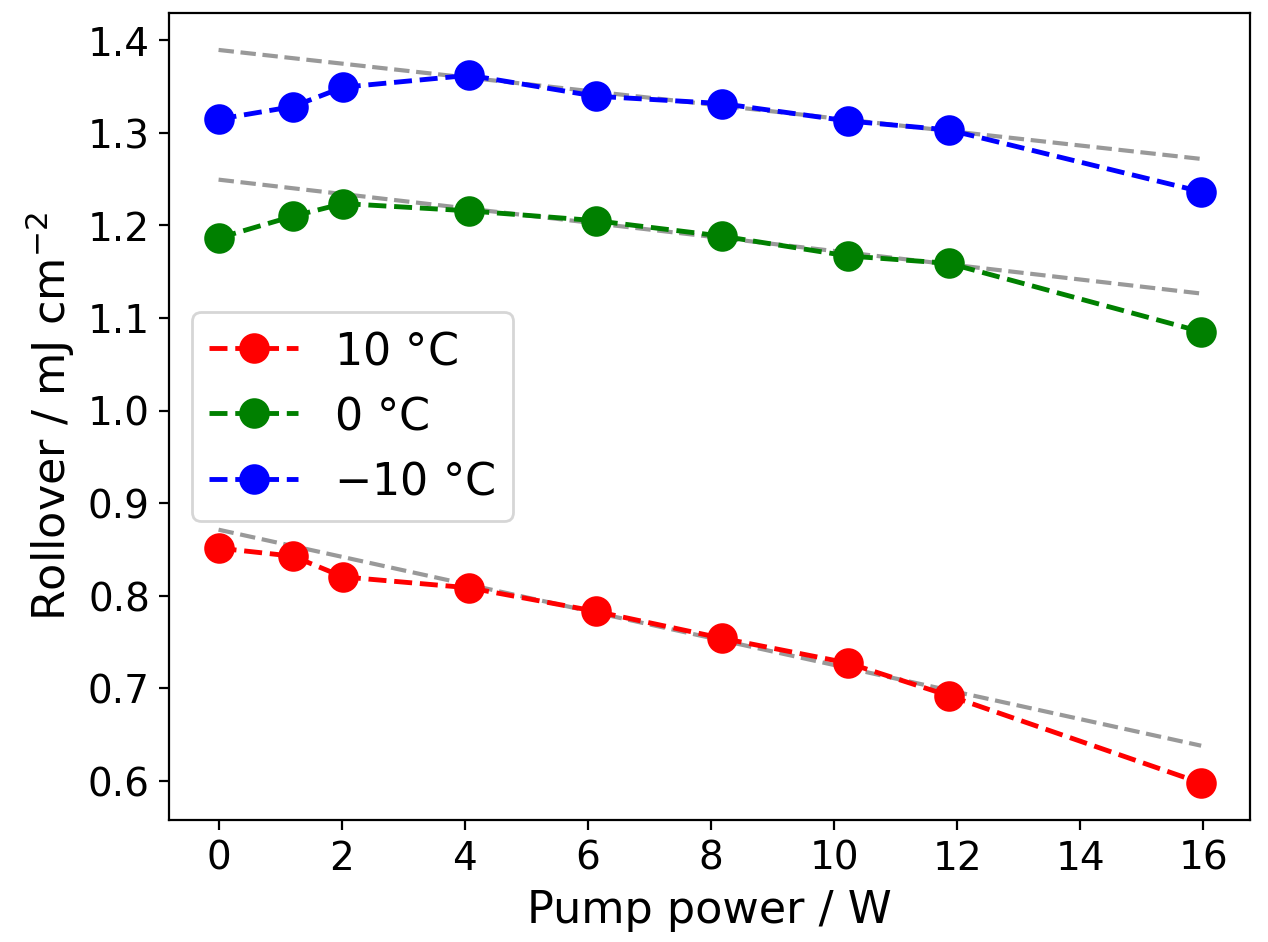
\includegraphics[width=.98\textwidth]{images/param3.png}
    \caption{Rollover parameter for the copper heat spreader pump DBR VECSEL with linear fits.}
    \label{fig:f2}
\end{wrapfigure}
In \cref{fig:f2} one can see the rollover parameter for the cDBR VECSEL. After reaching population inversion, we see a linear decrease of the rollover parameter for higher pump powers. This decrease in the rollover means, that for higher pump powers, we get a higher likelyhood of two photon absorption in the active region. This could be explained by the heating of the active region from the pump and the increase of the two-photon absorption rate with temperature.

As for the temperature dependence we see that we have a higher value for colder temperatures, which also aligns with the temperature dependence of the two-photon absorption. This behaviour of the two-photon absorption rate has also been previously observed in GaInAs \cite{GaAsTemp}.
\vspace{-\baselineskip}
\subsection*{Discussion}

In \cref{tab:f2} the fit parameters of a linear fit ($mx+b$) are listed for the different VECSEL chips and heat sink temperature. For the fit, we excluded the first three points, as we did for the saturation. If we compare the slopes of the different fits, no clear trend is observable, except that the slope has a negative sign.

Comparing the no pump DBR VECSEL with the pump DBR VECSEL we see that the no pump DBR VECSEL has almost double the rollover value. 

\begin{table}[ht]
    \centering
    \begin{tabular}{lllllllll}
        \hline
        Heat sink temperature & \multicolumn{2}{c}{\qty{10}{\celsius}} &      & \multicolumn{2}{c}{\qty{0}{\celsius}} &              & \multicolumn{2}{c}{\qty{-10}{\celsius}}                          \\ \cline{2-3} \cline{5-6} \cline{8-9}
        linear fit parameters & $m\cdot10^3$                           & $b$  &                                       & $m\cdot10^3$ & $b$                                     &  & $m\cdot10^3$ & $b$  \\ \hline
        No pump DBR           & -15.16                                 & 1.83 &                                       & -18.47       & 2.68                                    &  & -19.50       & 2.96 \\ \hline
        Copper, pump DBR      & -14.62                                 & 0.87 &                                       & -7.71        & 1.25                                    &  & -7.38        & 1.39 \\ \hline
        Diamond, pump DBR     & -9.21                                   & 0.93 &                                       & -5.19         & 1.54                                    &  & +5.62         & 1.55 \\ \hline
        Hybrid                & -0.35                                  & 5.33 &                                       & -21.1       & 2.72                                    &  & -7.98        & 2.23
    \end{tabular}
    \caption{Linear fit parameters of the saturation fluence. }
    \label{tab:f2}
\end{table}
\vspace{-2\baselineskip}

\section{Comparision to previous work}

If we want to compare our results to previous work. We can only do that for the no pump DBR VECSEL, since for the other structures no gain saturation measurements were done before. We can look at the work of Marco Gaulke et al. \cite{Gaulke2021HighCharacterization}. There results and ours can be seen in \cref{tab:comp}. 
The fit parameters indicating consistency between the two studies. We also observe the same constant behavior between saturation fluence and pump power as reported in the paper. 

Moreover, our investigation highlights a notable advancement in small signal gain for the new structure incorporating a pump DBR and diamond heat spreader. We achieve a record small signal gain of \qty{6.5}{\percent}, surpassing the previously reported value of \qty{3.5}{\percent}. This improvement signifies the enhanced performance and potential of the new structure in achieving higher gain.
\begin{table}[ht]
    \begin{tabular}{lcc}
        \cline{2-3}
                                                                      & previous work at 5 °C & this work at 10 °C \\ \hline
        Saturation fluence $F_{sat}$ / \unit{\micro\J\per\cm\squared} & 2.06 ± 0.11                                                                          & 1.9 ± 0.2                                                                        \\\hline
        Small signal Reflectivity $R_{ss}$ / \%                       & 103.5                                                                                & 102.5                                                                            \\\hline
        Nonsaturable reflectivity $R_{ns}$ / \%                       & 0.98 ± 0.12                                                                          & 0.99                                                                             \\\hline
        Rollover parameter $F_{2}$ / \unit{\micro\J\per\cm\squared}  & 2.01 ± 0.065                                                                         & 1.83
    \end{tabular}
    \caption{Comparison of the no pump DBR VECSEL parameters to the previous work of Marco Gaulke et al. \cite{Gaulke2021HighCharacterization}.\vspace{-1\baselineskip}}
    \label{tab:comp}
\end{table}   